\section{量子 K-理论（Xiaohan Yan 与 You-Cheng Chou）}%
\label{sec:Quantum K-theory (Xiaohan Yan and You-Cheng Chou)}

\subsection{概述}%
\label{sub:Overview}

Gromov–Witten 不变量是``计数''光滑射影簇 \(X\) 中曲线的一种方式。GW 理论给出形如
\[ \ab<\alpha_1, \ldots, \alpha_n>_{g, n, \beta} \in \Q \]
的数，其中 \(\alpha_i \in H^*(X)\) 为各种上同调类，\(g\) 为亏格，\(n\) 为标记点个数，\(\beta \in H_2(X, \Z)\) 为曲线类。它已被用于研究镜面对称，而在镜面对称之外也产生了一些双有理不变量。我们现在的目标是把这整个故事提升到 K-理论。量子 K-理论给出数
\[ \ab<V_1, \ldots, V_n>_{g, n, \beta} \in \Z \]
其中 \(V_1, \ldots, V_n \in K(X)\)。它们满足各种差分方程\footnote{可与上同调中的微分方程相比较。}，并已在三维镜面对称与表示论中找到各种应用。

\subsection{K-理论}%
\label{sub:K-theory}

\begin{defn}
    设 \(X\) 为光滑射影簇。则 \(X\) 的 \textit{K-理论} \(K(X)\) 是 \(X\) 上向量丛的 Grothendieck 群，其关系为：若
    \[ 0 \to V_1 \to V_2 \to V_3 \to 0 \]
    是短正合序列，则 \(V_2 = V_1 + V_3\)。
\end{defn}

\begin{rmk}\leavevmode
    \begin{enumerate}
        \item \(K(X)\) 在直和与张量积运算下是一个环；
        \item 陈特征标给出同构 \(K(X) \to A^*(X)\)，至少在 \(\Q\) 上工作时如此。
    \end{enumerate}
\end{rmk}

\begin{exm}
    设 \(X = \P^n\) 并记 \(P = \mc{O}(-1)\)。则我们有
    \[ K(X) = \C[P^{\pm 1}]/(P-1)^{n+1} \xrightarrow{\on{ch}} A^*(X) = \C[H]/H^{n+1}. \]
\end{exm}

对于不假定光滑的 Deligne–Mumford 栈，有两个版本
\[ K_0(X) \supset K^0(X), \]
其中 \(K_0\) 指凝聚层，\(K^0\) 指完美复形。二者在光滑射影簇上相同，因此从现在起 \(K(X)\) 均指 \(K_0(X)\)。存在张量积
\[ K^0(X) \otimes K_0(X) \to K_0(X) \]
以及沿本征态射的推出
\[ f_* \colon K(X) \to K(Y) \qquad V \mapsto \sum (-1)^i R^i f_* V \]
若 \(f\) 是完美态射（例如平坦、正则嵌入等），则存在拉回
\[ f^* \colon K(Y) \to K(X) \qquad W \mapsto \sum (-1)^i \on{Tor}_i^{f^{-1} \mc{O}_Y} (\mc{O}_X, f^{-1} W). \]

\subsection{曲线的模空间}%
\label{sub:Moduli of curves}

回忆到 \(X\) 的稳定映射的模空间
\[ \bar{M}_{g,n}(X, \beta) = \ab\{ f \colon (\Sigma, p_1, \ldots, p_n) \to X \mid g(\Sigma) = g, f_*[\Sigma] = \beta, \abs{\Aut f} < \infty \} \]
它有赋值映射
\[ \ev_i \colon \bar{M}_{g,n}(X, \beta) \to X \qquad (f, \Sigma, \ul{p}) \mapsto f(p_i). \]
还有万有余切线 \(L_i = \sigma_i^* \omega_{ \mc{C}/\bar{M} }\)。

该模空间是本征的 Deligne–Mumford 栈，并具有完美障碍理论，由此产生虚拟结构层 \(\mc{O}^{\vir}_{g,n,\beta}\)。它来自\textit{虚拟切丛}的结构，其中
\[ \mathbb{T}_{(f, \Sigma, \ul{p})} \bar{M}_{g,n}(X, \beta) = \chi(\Sigma, f^* T_X) - \chi(\Sigma, T_{\Sigma}(-p_1 - \cdots - p_n)). \]
粗略地说，若 \(\bar{M}\) 是簇 \(Y\) 上某向量丛 \(E\) 的一个截面的零轨迹，则 \(\mc{O}^{\vir} = \mc{O}_Y \otimes \mr{Eu}(E)\)，其中 K-理论 Euler 类为 \(\mr{Eu}(E) = \sum (-1)^i \Lambda^i E^{\vee}\)。

\subsection{KGW 不变量}%
\label{sub:KGW invariants}

关于量子 K-理论，见~\cite{Lee2004}；关于置换等变理论，见~\cite{Givental2017K1,GiventalK7}。To\"en~\cite{Toen1999} 证明了下面用到的 Deligne–Mumford 栈的 Riemann–Roch 公式。

\begin{defn}
    K-理论 GW 不变量定义为
    \[ \ab<V_1, \ldots, V_n>_{g,n,\beta} \coloneqq \chi\ab(\bar{M}_{g,n}(X, \beta); \mc{O}^{\vir} \otimes \bigotimes_{i=1}^n \ev_i^* V_i). \]
\end{defn}

若 \(V_1, \ldots, V_n\) 是真正的向量丛，则该不变量是整数，但一般地我们将考虑系数在特征零域中的 \(K_0\)。我们还可以定义引力后裔
\[ \ab<V_1 L_1^{k_1}, \ldots, V_n L_n^{k_n}>_{g,n,\beta} \coloneqq \chi\ab(\bar{M}_{g,n}(X, \beta); \mc{O}^{\vir} \otimes \bigotimes_{i=1}^n ( \ev_i^* V_i )L_i^{k_i} ). \]
利用由置换标记点给出的 \(S_n\) 在 \(\bar{M}_{g,n}(X, \beta)\) 上的作用，对象 \(\bigotimes_{i=1}^n \ev_i^* V\) 与 \(\bigotimes_{i=1}^n L_i^k\) 是 \(S_n\)-等变的。

\begin{defn}
    我们定义\textit{置换不变的 K-理论 GW 不变量}为
    \begin{align*}
        \ab<V L_1^k, \ldots, V L_n^k>_{g,n,\beta}^{S_n} &\coloneqq \chi\ab([ \bar{M}_{g,n}(X, \beta)/S_n ]; \mc{O}^{\vir} \otimes \bigotimes_{i=1}^n ( \ev_i^* V ) L_i^k) \\
        &= \dim \chi_{S_n} \ab(\bar{M}_{g,n}(X, \beta); \mc{O}^{\vir} \otimes \bigotimes_{i=1}^n ( \ev_i^* V ) L_i^k )^{S_n}.
    \end{align*}
\end{defn}

给定 \(t(q) = \sum_{n \in \Z} t_n q^n \in K(X)[q,q^{-1}]\)，我们可以定义
\[ \ab< t(L_1), \ldots, t(L_n)>^{S_n}_{g,n,\beta} \coloneqq \chi ([\bar{M}_{g,n}(X,\beta)/S_n], \cdots). \]
更一般地，若 \(H = S_{a_1} \times \cdots \times S_{a_m} \subset S_n\)，我们可以定义
\[ \ab<t_1(L_1), \ldots, t_1(L_{a_1}), t_2(L_{a_1+1}), \ldots, t_2(L_{a_1+a_2}), \ldots>_{g,n,\beta}^H. \]

\begin{rmk}
    我们想讨论它与通常 GW 不变量的一些关系。回忆 Hirzebruch–Riemann–Roch 断言
    \[ \chi(M; V) = \int_M \on{ch}(V) \on{td}(T_M). \]
    当 \(M\) 是光滑 Deligne–Mumford 栈时，T\"oen 证明了公式
    \[ \chi(M; V) = \int_{IM} \wt{\on{ch}}(V) \wt{\on{td}}(T_M), \]
    其中 \(IM = M \times_{\Delta, M \times M, \Delta} M\) 是 \(M\) 的惯性栈，而波浪线表示取轨形陈特征标与 Todd 类。
\end{rmk}

\begin{exm}
    若 \(M = B\mu_r\)，则 \(IM = \bigsqcup_{g \in \mu_r} B \mu_r\)。若 \(M = \P(1, r)\) 是加权 \(\P^1\)，则 \(IM = M \sqcup \bigsqcup_{g \neq 1 \in \mu_r} B\mu_r\)。    
\end{exm}

\begin{exm}
    设 \(M = BG\)，其中 \(G\) 为有限 Abel 群，并设 \(V\) 为 \(BG\) 上的向量丛，这等同于 \(G\) 的一个表示。则 \(\chi(M, V) = \dim V^G\)。另一方面，我们有
    \[ \int_{IM} \wt{\on{ch}}(V) \cdot \wt{\on{td}}(T_M) = \int_{IM} \on{tr}_g V = \sum_{g \in G} \frac{1}{\abs{G}} \on{tr}_g V = \dim V^G, \]
    因此我们在此情形下验证了 Riemann–Roch。
\end{exm}

\subsection{公理性质}%
\label{sub:Axiomatic properties}

\begin{lem}[{\cite{GiventalK7}}]
    我们有\textit{弦方程}
    \begin{align*}
        \ab< 1, x_1(L), \ldots, x_k(L), t, \ldots, t >_{g, 1+k+n, \beta}^{S_n} = \ab<x_1(L), \ldots, x_k(L), t^{\otimes n}>^{S_n}_{g,k+n,\beta} \\
        + \sum_i \ab< \cdots, \frac{x_i(L) - x_i(1)}{L-1}, \ldots, t^{\otimes n}>^{S_n}_{g,k+n,\beta}. 
    \end{align*}
\end{lem}

\begin{proof}
    证明与 GW 理论中相同，来自沿映射 \(\pi \colon\bar{M}_{g,n+1}(X,\beta) \to \bar{M}_{g,n}(X,\beta)\) 计算 \(\pi^* L_i\)。
\end{proof}

\begin{lem}[{\cite{GiventalK7}}]
    我们有\textit{胀子方程}
    \begin{align*}
        \ab<L-1, x_1(L), \ldots, x_k(L), t^{\otimes n}>_{g,1+k+n,\beta}^{S_n} ={}& (k-2)\ab<x_1(L), \ldots, x_k(L), t^{\otimes n}>_{g,k+n,\beta}^{S_n} \\
        &+ \ab<x_1(L), \ldots, x_k(L), t, t^{\otimes n-1}>_{g,k+n,\beta}^{S_{n-1}}.
    \end{align*}
\end{lem}

\begin{proof}
    我们利用事实
    \[ \pi_* L = k + \on{Ind}_{S_{n-1}}^{S_n}(1) - 1, \]
    其中 \(\pi\) 遗忘第一个标记点，而 \(L = \omega_{\pi} (p_1 + \cdots + p_n)\)。这由如下事实推出：存在留数映射
    \[ H^0(L) \xrightarrow{\on{Res}} \bigoplus_{i=1}^{k+n} \C p_i \xrightarrow{\sum} \C. \]
    中间项是 \(k\) 个平凡表示与一个标准表示的直和。
\end{proof}

\begin{notn}
    固定 \(\tau, t \in K(X)\)。我们记
    \[ \ab<\!\ab<x_1(L_1), \ldots, x_k(L_k)>\!>_{g,k} \coloneqq \sum_{m,n,\beta} \frac{Q^{\beta}}{m!} \ab<x_1(L_1), \ldots, x_k(L_k), \tau^{\otimes m}, t^{\otimes n}>_{g,k+m+n,\beta}^{S_n}. \]
    我们令 \(\{\phi_{\alpha}\}\) 为 \(K(X)\) 的一组基，\(\{\phi^{\alpha}\}\) 为其对偶基。然后定义配对
    \[ g_{\alpha\beta} = \chi(X, \phi_{\alpha} \otimes \phi_{\beta}). \]
    这并不完全是正确的配对，因此我们将考虑
    \[ G_{\alpha\beta} = g_{\alpha\beta} + \ab<\!\ab<\alpha,\beta>\!>_{0,2}. \]
    我们令 \(g^{\alpha\beta} = (g_{\alpha\beta})^{-1}\)，\(G^{\alpha\beta} = (G_{\alpha\beta})^{-1}\)。
\end{notn}

\begin{lem}[{\cite{Givental2000K}}]
    给定 \(A,B,C,D \in K(X)[q,q^{-1}]\)，我们有 \textit{WDVV 方程}
    \begin{align*}
        \sum_{\alpha,\beta} \ab<\!\ab< A(L), B(L), \phi_{\alpha}>\! >_{0,3}& G^{\alpha\beta}\ab<\!\ab< C(L), D(L), \phi_{\beta}>\! >_{0,3} \\
        &= \sum_{\alpha,\beta} \ab<\!\ab< A(L), C(L), \phi_{\alpha}>\! >_{0,3} G^{\alpha\beta}\ab<\!\ab< B(L), D(L), \phi_{\beta}>\! >_{0,3}. 
    \end{align*}
\end{lem}

\begin{proof}
    拉回 \(\bar{M}_{0,4} = \P^1\) 上边界除子的等式。在 K-理论中，当 \(D = \bigcup C_i\) 时，将 \(\mc{O}_D\) 与 \(\mc{O}_{C_i}\) 联系起来需要应用容斥原理，这正是 \(G^{\alpha\beta}\) 出现的原因。
\end{proof}

\subsection{圈空间形式体系}%
\label{sub:Loop space formalism}

\begin{defn}
    \textit{圈空间} \((\mc{K}, \Omega)\) 由
    \[ \mc{K} = K(X)(q) \ps{Q}\]
    连同辛形式
    \[ \Omega(f, g) = - \on{Res}_{q = 0, \infty} \ab<f(q^{-1}), g(q)>_X \frac{\d{q}}{q}. \]
    组成。
\end{defn}

\begin{rmk}
    存在极化 \(\mc{K} = \mc{K}_+ \oplus \mc{K}_-\)，其中
    \[ \mc{K}_+ = K(X)[q, q^{-1}]\ps{Q} \]
    而
    \[ \mc{K}_- = \ab\{ \frac{f}{g} \mid f, g \in K(X)\ps{Q}[q], g(0) \neq 0, \deg f < \deg g\}. \]
    例如，\(\frac{1}{1-q} \in \mc{K}_-\)。
\end{rmk}

\begin{defn}
    \textit{大 J-函数} \(J \colon \mc{K}_+ \to \mc{K}\) 由
    \[ \mathbf{t} = \mathbf{t}(q) \mapsto 1 - q + \mathbf{t}(q) + \sum_{\beta, \alpha} Q^{\beta} \phi^{\alpha} \ab< \frac{\phi_{\alpha}}{1-qL}, \mathbf{t}(L)^{\otimes n}>_{0, 1+n, \beta}^{S_n}. \]
    给出。
\end{defn}

\begin{rmk}
    注意到应用 Riemann–Roch，我们有
    \begin{align*}
        \chi\ab([\bar{M}/S_n], \frac{1}{1-qL}) &= \int_{I[\bar{M}/S_n]} \on{ch}\ab(\frac{1}{1-qL}) \on{td}.
    \end{align*}
    每一项都变为形如 \(\on{ch}\ab(\on{tr}_g \frac{1}{1-qL})\) 的东西，这给出形如 \(\on{ch}\ab(\frac{1}{1-q\zeta L})\) 的项，其中 \(\zeta\) 为某个单位根。然后我们可以展开
    \[ \frac{1}{1-q\zeta L} = \frac{1}{(1-q \zeta) - q\zeta (L-1)} = \sum_k \frac{(q\zeta)^k}{(1-q\zeta)^{k+1}}(L-1)^k. \]
\end{rmk}

\begin{defn}
    \textit{Givental 锥}定义为 \(\mc{L} \coloneqq \Ima J \subset \mc{K}\)，其中我们考虑的是在 \(Q\)-进拓扑下 \(1-q\) 附近的芽。
\end{defn}

\begin{exm}
    设 \(X = \P^n\)。则我们看到
    \[ J(0) = (1-q) \sum_{d \geq 0} \frac{Q^d}{\prod_{\ell=1}^d (1-Pq^{\ell})^{n+1}}, \]
    其中 \(P = \mc{O}(-1)\)。同前，我们可以展开
    \[ \frac{1}{1-P q^{\ell}} = \frac{1}{(1-q^{\ell}) - q^{\ell}(P-1)} = \sum_{k=0}^{\infty} \frac{q^{\ell k}}{(1-q^{\ell})^{k+1}}(P-1)^k. \]
\end{exm}

\begin{prop}[{\cite{GiventalK7}}]
    事实上，\(\mc{L}\) 确实是 \(\mc{K}\) 中的一个锥，并且我们有
    \[ \mc{L} = \bigcup_{t \in K(X)\ps{Q}} (1-q) S_{t}^{-1}(q) \mc{K}_+. \]
\end{prop}

我们还可以引入一个``巨大''的 J-函数
\[ J(\mathbf{t}, \tau) = 1-q + \mathbf{t}(q) + \tau + \sum_{\beta, k, \alpha} \frac{Q^{\beta}}{k!} \phi^{\alpha} \ab< \frac{\phi_{\alpha}}{1-qL}, \mathbf{t}(L)^{\otimes n}, \tau^{\otimes k}>_{0,1+n+k,\beta}^{S_n}. \]
若固定 \(\mathbf{t}(q)\)，则 \(J(\tau)\) 来自关于 \(\tau\) 的 Frobenius 流形上某个\textit{微分方程}的基本解。此外，\(\mc{L}^{\mathbf{t}}=  \Ima J(\tau)\) 实际上是一个 Lagrange 锥。

\begin{exm}
    考虑由 Adams 运算给出的 \(f \colon \C[\Lambda_1^{\pm}, \Lambda_2^{\pm}] \to \C[\Lambda_1^{\pm}, \Lambda_2^{\pm}]\)：
    \[ t \mapsto \on{tr}_{(1\cdots n)} t^{\otimes n} = \Psi^n (t). \]
    因此它把 \(\Lambda_1 \mapsto \Lambda_1^n\)，\(\Lambda_2 \mapsto \Lambda_2^n\)。然而，如何对 \(t\) 求导并不清楚，因为我们需要 \(nv t^{n-1} = \Psi^n(v)\)，所以 J-函数不满足关于 \(\mathbf{t}\) 的量子微分方程。
\end{exm}

\subsection{等变 K-理论与局部化}%
\label{sub:Equivariant K-theory and localization}

关于不动点递归与射影空间的计算，见~\cite{GiventalK2}。

设环面 \(T = (\C^{\times})^r\) 作用在光滑射影簇 \(X\) 上。

\begin{defn}
    \textit{等变 K-理论} \(K_T(X)\) 是 \(X\) 上 \(T\)-等变向量丛的 Grothendieck 群。
\end{defn}

\begin{exm}
    例如，我们有
    \[ K_T(\on{pt}) = \on{Rep}(T) = \C[\Lambda_1^{\pm}, \ldots, \Lambda_r^{\pm}], \]
    其中 \(\Lambda_i\) 是权为 \((0, \ldots, 1, \ldots, 0)\) 的 \(1\) 维表示。
\end{exm}

\begin{rmk}
    对任意 \(X\)，\(K_T(X)\) 是一个 \(K_T(\mr{pt})\)-代数。
\end{rmk}

\begin{exm}
    考虑 \(\P^n\) 的完全等变 K-理论。则我们有
    \[ K_T(\P^n) = \C[P^{\pm}, \Lambda_0^{\pm}, \ldots, \Lambda_n^{\pm}] \big/ \prod_{i=0}^n (P-\Lambda_i). \]
    当我们代入 \(\Lambda_i = 1\) 时，便恢复出非等变 K-理论。
\end{exm}

\begin{defn}
    我们可以把等变 Euler 特征定义为推出
    \[ \chi_T = \pi_* \colon K_T(X) \to K_T(\mr{pt}). \]
\end{defn}

\begin{exm}
    例如，我们有 \(\chi_T(\mc{O}_{\P^1}(1)) = \Lambda_0^{-1} + \Lambda_1^{-1}\)。类似地，我们有
    \[ \chi_T(\mc{O}(2)) = \Lambda_0^{-2} + \Lambda_0^{-1} \Lambda_1^{-1} + \Lambda_1^{-2}. \]
\end{exm}

\begin{notn}
    注意到 \(\on{Frac}(T) = \on{Frac}(\on{Rep}(T))\)。然后我们记
    \[ K_T^{\loc}(X) \coloneqq \on{Frac}(T) \otimes_{\on{Rep}(T)} K_T(X). \]
\end{notn}

我们将需要如下事实。设 \(F\) 为 \(T\) 在 \(X\) 上的不动点集，并考虑 \(\iota \colon F \hookrightarrow X\)。则有 \(\on{Frac}(T)\)-代数的同构
\[ K_T^{\loc}(X) \xrightarrow{\iota^*} K_T^{\loc}(F). \]

\begin{rmk}
    其逆由
    \[ (\iota^*)^{-1} = \bigoplus_{i=1}^r \frac{\iota_{i*}}{\on{Eu}(N_{F_i/X})}, \]
    给出，其中 \(\on{Eu}(V) \coloneqq \sum_{j = 0}^{\on{rk} V} (-1)^j \Lambda^j V^*\) 是 K-理论 Euler 类。
\end{rmk}

\begin{exm}
    在 \(\P^n\) 上，我们有 \(n+1\) 个孤立不动点 \(F_i\)，于是我们得到
    \[ \frac{\iota_{i*} \mc{O}_{F_i}}{\on{Eu}(N_{F_i/\P^n})} = \prod_{j \neq i} \frac{P - \Lambda_j}{\Lambda_i - \Lambda_j}. \]
    它们是 \(K_T^{\loc}(\P^n)\) 的幂等元。
\end{exm}

利用等变局部化，我们得到
\[ \chi_T(X; V) = \sum_i \chi\ab(F_i; \frac{\iota_i^* V}{\on{Eu}(N_{F_i/X})}). \]

\begin{rmk}
    在 \(\Lambda = 1\) 的极限下，我们可以恢复出非等变 Euler 特征。
\end{rmk}

\begin{exm}
    设 \(X = \P^1\)。则我们计算
    \begin{align*}
        \chi_T(\P^1, \mc{O}(1)) &= \chi\ab(F_0, \frac{\mc{O}(1)|_{F_0}}{\on{Eu}(T_{F_0/\P^1})}) + \chi\ab(F_1, \frac{\mc{O}(1)|_{F_1}}{\on{Eu}(T_{F_1/\P^1})}) \\
        &= \frac{\Lambda_0^{-1}}{1 - \frac{\Lambda_0}{\Lambda_1}} + \frac{\Lambda_1^{-1}}{1 - \frac{\Lambda_1}{\Lambda_0}} \\
        &= \Lambda_0^{-1} + \Lambda_1^{-1}. 
    \end{align*}
\end{exm}

从现在起，我们将假设 \(X\) 是 GKM 流形。我们现在的目标是利用 \(\bar{M}_{g,n}(X, \beta)\) 上的局部化来研究 \(X\) 的大 J-函数。任何 \(T\)-不动的稳定映射 \(f \colon (\Sigma, \ul{p}) \to X\) 都有两类不可约分支：一类分支整个映入不动点，另一类分支经由 \(1\) 维轨道的分歧覆叠映入。遗憾的是，我们无法通过虚拟局部化来计算大 J-函数，但仍可以对它进行研究。

设 \(f = f(q) \in \mc{K} = K_T^{\loc}(X)(q)\ps{Q}\)。记不动点为 \(F_{\alpha}\)，\(\alpha = 1, \ldots, r\)，其包含映射为 \(\iota_{\alpha} \colon F_{\alpha} \hookrightarrow X\)。然后记
\[ f_{\alpha}(q) = \iota_{\alpha}^* f(q) \in K_T^{\loc}(\on{pt})(q)\ps{Q}. \]
则 \(f \in \mc{L}\) 当且仅当对所有 \(\alpha\)，以下条件成立：
\begin{enumerate}
    \item 给定 \(\lambda \in T_{F_{\alpha}} X\) 与 \(m \in \N_+\)，\(f_{\alpha}(q)\) 在 \(q = \lambda^{1/m}\) 处至多有单极点，并且
        \[ \on{Res}_{q = \lambda^{1/m}} f_{\alpha}(q) \frac{\d{q}}{q} = -\frac{Q^m}{m} \cdot \frac{\on{Eu}(T_{F_{\alpha}/X})}{\on{Eu}(T^{\vir}_{\phi_{\alpha,\alpha',m}}\bar{M}_{0,2}(X, m \cdot \beta(\alpha, \alpha')))} \cdot f_{\alpha'}(\lambda^{1/m}). \]
        这里，\(\lambda \in T_{F_{\alpha}}X\) 意指 \(\lambda\) 是 \(T_{F_{\alpha}} X\) 的一个 \(1\) 维子表示。此外，\(\beta(\alpha,\alpha')\) 是由权 \(\lambda\) 确定的 \(T\) 的 \(1\) 维轨道的次数，而 \(\phi_{\alpha, \alpha', m}\) 参数化该 \(1\) 维轨道的 \(m:1\) 覆叠。
    \item \(f_{\alpha}(q)\) 的其余极点位于 \(0\)、\(\infty\) 以及单位根处，在其他地方均正则。此外还有各种次要条件。
\end{enumerate}

\begin{exm}
    设 \(X = \P^n\)。则
    \[ J_T^X(0) = (1-q) \sum_{d \geq 0} \frac{Q^d}{\prod_{i=0}^n \prod_{\ell = 1}^d \ab(1 - \frac{P}{\Lambda_i} q^{\ell})} \in K_T(X)(q) \ps{Q}. \]
    于是这意味着
    \[ J_T^X(0) |_{F_j} = (1-q) \sum_{d \geq 0} \frac{Q^d}{\prod_{i=0}^n \prod_{\ell = 1}^d \ab(1 - \frac{\Lambda_j}{\Lambda_i}q^{\ell})}, \]
    所以极点位于 \(q = \ab(\frac{\Lambda_i}{\Lambda_j})^{1/\ell}\)。再注意到
    \[ T_{F_j} X = \frac{\Lambda_0}{\Lambda_j} + \cdots + \frac{\Lambda_n}{\Lambda_j} - 1. \]
\end{exm}

\subsection{量子 K/GV 对应}%
\label{sub:Quantum K/GV correspondence}

五次三维簇的对应猜想于~\cite{GaroufalidisScheidegger2022}，并在~\cite{ChouLeeQuintic} 中得到证明。下面的 Calabi–Yau 三维簇公式归功于 Chou–Lee~\cite{ChouLee2025}。

我们在此的目标是在 Calabi–Yau 三维簇上计算 \(J^K(0)\)。下述结果曾由 Jockers–Mayr 以及 Garoufalidis–Scheidegger 猜想。

\begin{thm}[{\cite{ChouLee2025}}]
    我们有
    \begin{align*}
        J^K(0) &\coloneqq (1-q) + \sum_{\beta, \alpha} Q^{\beta} \Phi^{\alpha} \ab<\frac{\Phi_{\alpha}}{1-qL}>_{0,1,\beta}^{X,K} \\
        &= (1-q) + \sum_{\beta} \sum_{r=1}^{\infty} \mr{GV}_{\beta} Q^{r\beta} \ab[\sum_{j=1}^{n_1} \Phi^{1j} a(r, q^r) + \Phi^{01} b(r, q^r)],
    \end{align*}
    其中 \(\ab\{\Phi_{\alpha}\}_{\alpha=1}^N\) 是 \(K^0(X)\) 的一组基，分解为
    \[ \ab\{\Phi_{\alpha}\}_{\alpha=1}^N = \bigsqcup_{i=0}^3 \ab\{\Phi_{ij}\}_{j=1}^{n_i} \]
    使得对固定的 \(i\)，\(\ch(\Phi_{ij})\) 构成 \(H^{2i}(X)\) 的一组基。然后我们选取对偶基 \(\ab\{\Phi^{\alpha}\}_{\alpha} = \ab\{\Phi^{ij}\}_{i,j}\)。此外，我们设定多重覆叠公式
    \begin{align*}
        a(r, q^r) &= \frac{r-1}{1-q^r} + \frac{1}{(1-q^r)^2}, \\
        b(r, q^r) &= \frac{r^2-1}{1-q^r} + \frac{3}{(1-q^r)^2} - \frac{2}{(1-q^r)^3}.
    \end{align*}
    最后，GV 表示 Gopakumar–Vafa 不变量，在亏格零时定义为
    \[ \mr{GW}_{0,\beta} = \sum_{r \mid \beta} \frac{1}{r^3} \mr{GV}_{\beta/r}. \]
    由 M\"obius 反演，我们看到
    \[ \mr{GV}_{\beta} = \sum_{r \mid \beta} \frac{\mu(r)}{r^3} \mr{GW}_{0,\beta/r}. \]
\end{thm}

\begin{cor}[{\cite{ChouLee2025}}]
    我们有
    \[ \ab<1>_{0,1,\beta}^K = \sum_{r \mid \beta} r^2 \mr{GV}_{\beta/r}. \]
    应用 M\"obius 反演，我们得到\footnote{注意，该结果在所有亏格下已由 Ionel–Parker~\cite{IonelParker2018} 得到。}
    \[ \mr{GV}_{\beta} = \sum_{r \mid \beta} r^2 \mu(r) \ab<1>_{0,1,\beta/r}^K \in \Z. \]
    此外，我们可以通过\footnote{这类似于：如果我们应用 Hirzebruch–Riemann–Roch 来计算 K-理论配对，最高次项只能看到两个输入的陈特征标。}
    \[ \lim_{q \to 1} (1-q)^3 \ab<\frac{1}{1-qL}>_{0,1,\beta}^{X,K} = \sum_{r \mid \beta} \frac{-2}{r^3} \mr{GV}_{\beta/r} = -2 \mr{GW}_{\beta} = \ab<\psi>_{0,1,\beta}^{\mr{GW}}. \]
    恢复出通常的 GW 不变量。
\end{cor}

朴素地看，我们可以认为 \(J^K(0) \in \Z\ps{q}\ps{Q}\)，但更精确一点，我们可以考虑
\[ J^K(0) \in 1-q + \mc{K}_-. \]
这里我们展开 \(\frac{1}{1-qL} = \sum q^i L^i\)。
我们还需要考虑如下事实：若 \(M\) 是 Deligne–Mumford 栈，\(L\) 是 \(M\) 上的线丛，则函数
\[ f^{\Phi}(q) \coloneqq \chi\ab(M, \frac{\Phi}{1-qL}) \in \Z \ps{q} \]
在 \(\abs{q} < \ep\) 时收敛于一个有理函数。注意极点只出现在单位根处。

这一事实可以用轨形 Riemann–Roch 定理证明。把惯性栈分解为
\begin{align*}
    IM &= \bigsqcup_{i \in I} M_i \\
    &= \bigsqcup_{\zeta} M_{\zeta},
\end{align*}
其中 \(M_{\zeta}\) 是使得 \(g\) 以特征值 \(\zeta\) 作用在 \(L\) 上的扭曲扇区的并。利用这一点，我们可以计算
\begin{align*}
    \chi\ab(M, \frac{1}{1-qL}) &= \sum_{i \in I} \int_{M_i} \on{td}(M_i) \on{ch} \ab(\frac{ \on{Tr}_g \ab(\frac{1}{1-qL}) }{\lambda_{-1}(N_{M_i/M}^*)}) \\
    &= \sum_{\zeta} \int_{M_{\zeta}} \on{td}(M_{\zeta}) \sum_{k \geq 0} \frac{(\zeta q)^k}{(1-\zeta q)^{k+1}} \frac{( \on{ch}(L)-1 )^k}{\ch \lambda_{-1}(N^*)},
\end{align*}
因此所有极点必定位于单位根处。这里我们用了展开式
\[ \frac{1}{1-\zeta q L} = \sum_{k \geq 0} \frac{(\zeta q)^k}{(1-\zeta q)^{k+1}} (L-1)^k \]
并取了陈特征标。

\begin{exm}
    设 \(L = \mc{O}(1)\) 于 \(\P^1\) 上。则我们有
    \begin{align*}
        \chi\ab(\P^1, \frac{1}{1-qL}) &= \chi\ab(\P^1, \frac{1}{1-q} + \frac{q}{(1-q)^2}(L-1)) \\
        &= \sum_{i \geq 0} q^i (i+1) \\
        &= \frac{1}{(1-q)^2}.
    \end{align*}
\end{exm}

\begin{exm}
    我们现在考虑加权射影空间。则我们有
    \begin{align*}
        \chi\ab(\P(w_0, \ldots, w_n), \frac{1}{1-qL}) &= \prod_{i=0}^n \frac{1}{1-q^{w_i}}. 
    \end{align*}
\end{exm}

\subsection{阿代尔刻画}%
\label{sub:Adelic characterization}

回忆在所有亏格下，GW 与 GV 不变量之间存在一个由显式公式给出的关系。另一方面，我们可以通过 \(q \to 1\) 的极限从 KGW 不变量恢复 GW 不变量。反方向则需要 Givental–Tonita 的\textit{阿代尔刻画}（adelic characterization）~\cite{GiventalTonita2014}。其想法是：若我们有一个有理函数 \(f\)，则可以从它在各单位根 \(\zeta\) 处的 Laurent 展开
\[ f_{q=\zeta} = \sum f_{\zeta, k} (1-\zeta^{-1} q)^k \]
把它恢复出来。

我们将研究惯性栈 \(I\bar{M}_{0,1}(X, \beta)\)。可以通过~\Cref{fig:givental-png} 或~\Cref{fig:adelic-components} 来记录其各分支。
\begin{figure}[htpb]
    \centering
    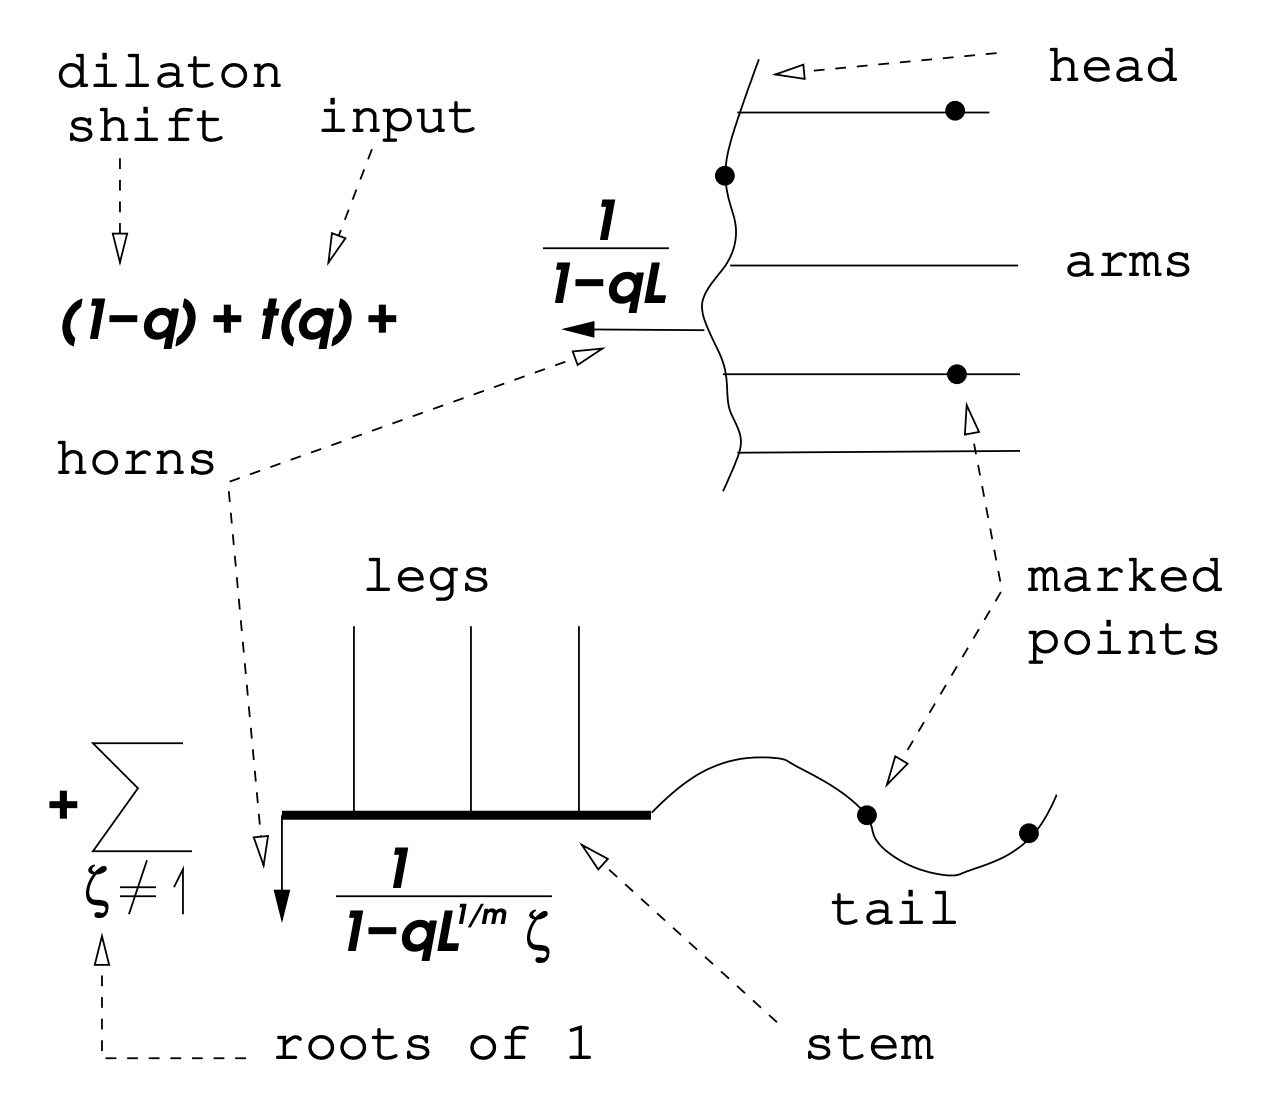
\includegraphics[width=0.8\textwidth]{givental.png}
    \caption{Givental–Tonita 给出的一种记录惯性栈各分支的方式。}
    \label{fig:givental-png}
\end{figure}

\begin{figure}[htpb]
    \centering
    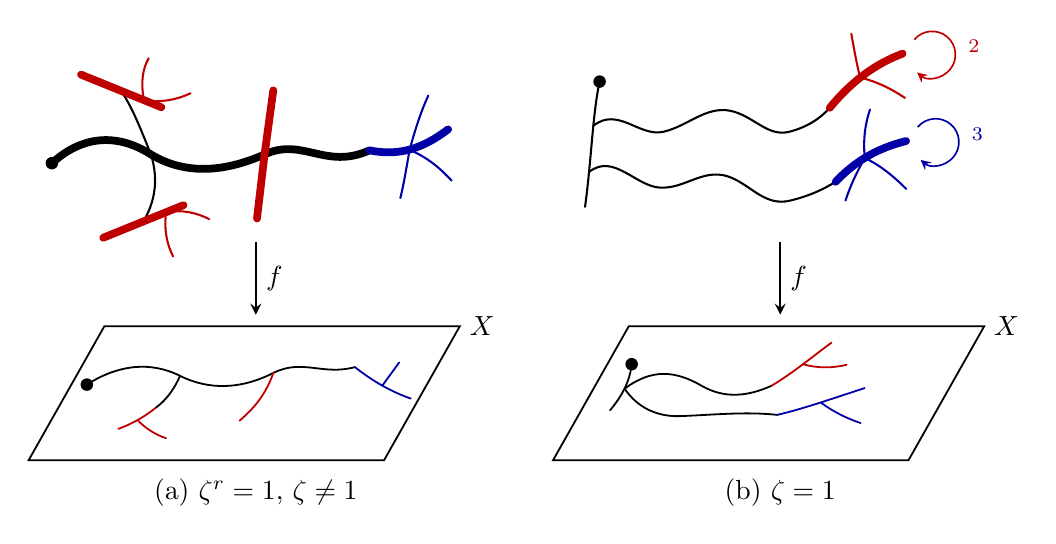
\begin{tikzpicture}[
        x=.74cm, y=.74cm,
        % Components of the domain curve. A cover style means the component
        % is a multiple cover of its image, drawn thick.
        dom/.style      ={black,         line width=.75pt, line cap=round},
        domcover/.style ={black,         line width=2.8pt, line cap=round},
        redcover/.style ={red!75!black,  line width=2.8pt, line cap=round},
        redtwig/.style  ={red!75!black,  line width=.75pt, line cap=round},
        bluecover/.style={blue!65!black, line width=2.8pt, line cap=round},
        bluetwig/.style ={blue!65!black, line width=.75pt, line cap=round},
        % Everything downstairs in X is drawn thin.
        img/.style      ={black,         line width=.65pt, line cap=round},
        redimg/.style   ={red!75!black,  line width=.65pt, line cap=round},
        blueimg/.style  ={blue!65!black, line width=.65pt, line cap=round},
        grparrow/.style ={->, >=stealth, line width=.6pt},
        fmap/.style     ={->, >=stealth, line width=.75pt},
        bull/.style     ={circle, fill=black, inner sep=1.6pt},
    ]

    %%%%%%%%%%%%%%%%%%%%%%%%%%%%%%%%%%%%%%%%%%%%%%%%%%%%%%%%%%%%%%%%%%%%%%%
    %% (a) zeta a primitive r-th root of unity, r >= 2.
    %%%%%%%%%%%%%%%%%%%%%%%%%%%%%%%%%%%%%%%%%%%%%%%%%%%%%%%%%%%%%%%%%%%%%%%
    \begin{scope}
        % The distinguished component: here g^r acts trivially on it, but g
        % does not, so it is a multiple cover of its image.
        \node[bull] at (-3.5,1.9) {};
        \draw[domcover]
            (-3.5,1.9)
            .. controls (-2.95,2.40) and (-2.35,2.40) .. (-1.80,2.05)
            .. controls (-1.25,1.72) and (-0.60,1.72) .. ( 0.15,2.05)
            .. controls ( 0.80,2.35) and ( 1.20,1.78) .. ( 1.95,2.12);

        % A leg meeting the distinguished component at a balanced node,
        % sticking out on both sides.  Each end carries a red multiple cover
        % together with the two branches interchanged by its automorphism.
        \draw[dom] (-1.80,2.05) .. controls (-2.00,2.55) and (-2.12,2.85) .. (-2.31,3.14);
        \draw[redcover] (-3.00,3.42) -- (-1.62,2.86);
        \draw[redtwig] (-1.92,2.98) .. controls (-1.98,3.30) and (-1.94,3.52) .. (-1.84,3.70);
        \draw[redtwig] (-1.92,2.98) .. controls (-1.62,2.94) and (-1.38,2.98) .. (-1.12,3.10);

        \draw[dom] (-1.80,2.05) .. controls (-1.66,1.60) and (-1.74,1.22) .. (-1.93,0.90);
        \draw[redcover] (-2.62,0.62) -- (-1.24,1.18);
        \draw[redtwig] (-1.54,1.06) .. controls (-1.58,0.74) and (-1.52,0.50) .. (-1.42,0.30);
        \draw[redtwig] (-1.54,1.06) .. controls (-1.26,1.10) and (-1.04,1.06) .. (-0.80,0.94);

        % A second balanced node, where the two legs are themselves the
        % multiple covers.
        \draw[redcover] (0.15,2.05) -- (0.30,3.15);
        \draw[redcover] (0.15,2.05) -- (0.02,0.95);

        % The tail: the part cut off at the unbalanced node.
        \draw[bluecover]
            (1.95,2.12) .. controls (2.45,2.02) and (2.85,2.14) .. (3.30,2.48);
        \draw[bluetwig] (2.64,2.13) .. controls (2.74,2.50) and (2.84,2.80) .. (2.96,3.06);
        \draw[bluetwig] (2.64,2.13) .. controls (2.58,1.80) and (2.54,1.54) .. (2.48,1.30);
        \draw[bluetwig] (2.64,2.13) .. controls (2.94,2.00) and (3.16,1.82) .. (3.36,1.60);

        \draw[fmap] (0,0.55) -- node[right] {$f$} (0,-0.70);

        % The target and the image of the map.
        \draw[img] (-3.9,-3.2) -- (2.2,-3.2) -- (3.5,-0.9) -- (-2.6,-0.9) -- cycle;
        \node[right] at (3.5,-0.9) {$X$};
        \node[bull] at (-2.90,-1.90) {};
        \draw[img] (-2.90,-1.90)
            .. controls (-2.35,-1.55) and (-1.80,-1.50) .. (-1.30,-1.75)
            .. controls (-0.80,-2.00) and (-0.25,-1.98) .. ( 0.30,-1.70)
            .. controls ( 0.80,-1.45) and ( 1.15,-1.75) .. ( 1.70,-1.60);
        % The two branches upstairs are folded onto the single one downstairs.
        \draw[img]    (-1.30,-1.75) .. controls (-1.42,-2.02) and (-1.56,-2.18) .. (-1.72,-2.30);
        \draw[redimg] (-1.72,-2.30) .. controls (-1.92,-2.46) and (-2.14,-2.58) .. (-2.36,-2.66);
        \draw[redimg] (-2.02,-2.52) .. controls (-1.88,-2.66) and (-1.72,-2.76) .. (-1.54,-2.82);
        \draw[redimg] ( 0.30,-1.70) .. controls ( 0.18,-2.05) and (-0.02,-2.30) .. (-0.28,-2.52);
        \draw[blueimg] (1.70,-1.60) .. controls (2.02,-1.85) and (2.32,-2.02) .. (2.66,-2.14);
        \draw[blueimg] (2.17,-1.92) .. controls (2.27,-1.78) and (2.36,-1.66) .. (2.46,-1.52);

        \node at (0,-3.75) {(a) \(\zeta^r = 1\), \(\zeta \neq 1\)};
    \end{scope}

    %%%%%%%%%%%%%%%%%%%%%%%%%%%%%%%%%%%%%%%%%%%%%%%%%%%%%%%%%%%%%%%%%%%%%%%
    %% (b) zeta = 1.
    %%%%%%%%%%%%%%%%%%%%%%%%%%%%%%%%%%%%%%%%%%%%%%%%%%%%%%%%%%%%%%%%%%%%%%%
    \begin{scope}[shift={(9,0)}]
        % Now g acts trivially on the distinguished component, so it is drawn
        % thin: it maps isomorphically onto its image.
        \node[bull] at (-3.10,3.30) {};
        \draw[dom] (-3.10,3.30) .. controls (-3.22,2.75) and (-3.24,1.95) .. (-3.35,1.15);
        \draw[dom] (-3.21,2.54)
            .. controls (-2.78,2.88) and (-2.42,2.34) .. (-2.00,2.44)
            .. controls (-1.58,2.54) and (-1.28,2.88) .. (-0.86,2.80)
            .. controls (-0.46,2.72) and (-0.22,2.34) .. ( 0.16,2.44)
            .. controls ( 0.46,2.52) and ( 0.68,2.66) .. ( 0.85,2.85);
        \draw[dom] (-3.28,1.75)
            .. controls (-2.86,2.08) and (-2.48,1.50) .. (-2.06,1.48)
            .. controls (-1.64,1.46) and (-1.34,1.80) .. (-0.92,1.68)
            .. controls (-0.52,1.56) and (-0.28,1.14) .. ( 0.18,1.26)
            .. controls ( 0.50,1.34) and ( 0.72,1.44) .. ( 0.95,1.58);

        % The arms: g acts nontrivially on them, through the indicated cyclic
        % group, which interchanges the thin branches sticking out.
        \draw[redcover] (0.85,2.85) .. controls (1.22,3.30) and (1.62,3.60) .. (2.10,3.78);
        \draw[redtwig] (1.37,3.37) .. controls (1.30,3.66) and (1.26,3.90) .. (1.22,4.12);
        \draw[redtwig] (1.37,3.37) .. controls (1.66,3.30) and (1.90,3.18) .. (2.14,3.02);
        \draw[grparrow, red!75!black]
            (2.30,4.02) arc[start angle=140, end angle=-130, radius=.40];
        \node[red!75!black, right] at (3.06,3.90) {$\Z_2$};

        \draw[bluecover] (0.95,1.58) .. controls (1.30,1.95) and (1.68,2.16) .. (2.16,2.28);
        \draw[bluetwig] (1.45,1.99) .. controls (1.42,2.32) and (1.46,2.58) .. (1.54,2.82);
        \draw[bluetwig] (1.45,1.99) .. controls (1.72,1.86) and (1.94,1.68) .. (2.16,1.46);
        \draw[bluetwig] (1.45,1.99) .. controls (1.30,1.72) and (1.20,1.50) .. (1.12,1.26);
        \draw[grparrow, blue!65!black]
            (2.36,2.52) arc[start angle=140, end angle=-130, radius=.40];
        \node[blue!65!black, right] at (3.12,2.40) {$\Z_3$};

        \draw[fmap] (0,0.55) -- node[right] {$f$} (0,-0.70);

        % The target and the image of the map.
        \draw[img] (-3.9,-3.2) -- (2.2,-3.2) -- (3.5,-0.9) -- (-2.6,-0.9) -- cycle;
        \node[right] at (3.5,-0.9) {$X$};
        \node[bull] at (-2.55,-1.55) {};
        \draw[img] (-2.55,-1.55) .. controls (-2.58,-1.85) and (-2.72,-2.10) .. (-2.92,-2.34);
        \draw[img] (-2.67,-1.97)
            .. controls (-2.20,-1.62) and (-1.80,-1.66) .. (-1.35,-1.92)
            .. controls (-0.95,-2.15) and (-0.55,-2.10) .. (-0.15,-1.92);
        \draw[img] (-2.67,-1.97)
            .. controls (-2.45,-2.30) and (-2.10,-2.46) .. (-1.70,-2.44)
            .. controls (-1.15,-2.42) and (-0.60,-2.36) .. (-0.05,-2.42);
        % Each arm is folded onto a single image curve with one branch.
        \draw[redimg] (-0.15,-1.92) .. controls (0.25,-1.68) and (0.55,-1.42) .. (0.88,-1.18);
        \draw[redimg] ( 0.39,-1.55) .. controls (0.63,-1.62) and (0.89,-1.62) .. (1.14,-1.56);
        \draw[blueimg] (-0.05,-2.42) .. controls (0.45,-2.30) and (0.95,-2.12) .. (1.45,-1.96);
        \draw[blueimg] ( 0.70,-2.21) .. controls (0.90,-2.36) and (1.14,-2.48) .. (1.38,-2.56);

        \node at (0,-3.75) {(b) \(\zeta = 1\)};
    \end{scope}
    \end{tikzpicture}
    \caption{\(I\bar{M}_{0,1}(X,\beta)\) 的各分支，归功于 You-Cheng。}
    \label{fig:adelic-components}
\end{figure}

我们现在解释~\Cref{fig:adelic-components}。设 \(L_1\) 为第一个标记点处的余切线，并设 \(g\) 为 \(I\bar{M}_{0,1}(X,\beta)\) 中某点的自同构。则 \(\zeta\) 由 \(g\) 以特征值 \(\zeta\) 作用在 \(L_1\) 上这一条件定义。在两幅图中，圆点表示第一个标记点及其在 \(X\) 中的像，而粗线分支表示其像的多重覆叠。

首先，设 \(\zeta = 1\)。此时黑色分支是包含第一个标记点且 \(g\) 在其上恒等作用的极大连通分支。红色与蓝色分支恰好是那些 \(g\) 在其上非平凡作用的分支，我们称之为\textit{臂}（arm）。

现在设 \(\zeta\) 是某个 \(r \geq 2\) 次单位根。此时要求黑色分支的结点关于 \(g\)-作用是平衡的，因此我们切去不平衡的部分，即着为蓝色的部分，并称之为\textit{尾}（tail）。在剩下的部分中，黑色分支是包含第一个标记点且 \(g^r\) 在其上恒等作用的极大连通分支。最后，去掉黑色分支与尾之后，我们称其余分支为\textit{腿}（leg）。

% \begin{figure}[htpb]
%     \centering
%     \resizebox{\textwidth}{!}{%
%     \begin{tikzpicture}[
%         x=1cm,
%         y=1cm,
%         curve/.style={black, line width=1.25pt, line cap=round},
%         fixed component/.style={black, line width=3.2pt, line cap=round},
%         red component/.style={red!75!black, line width=3.2pt, line cap=round},
%         blue component/.style={blue!70!black, line width=3.2pt, line cap=round},
%         image curve/.style={black, line width=1.05pt, line cap=round},
%         action arrow/.style={->, >=stealth, line width=.75pt},
%         map arrow/.style={->, >=stealth, line width=.8pt},
%         marked point/.style={circle, fill=black, inner sep=1.8pt}
%     ]
%         % The case of a nontrivial r-th root of unity.
%         \begin{scope}[xshift=0cm]
%             \node[font=\large] at (0,5.95)
%                 {$r\geq 2,\qquad \zeta^r=1,\quad \zeta\neq 1$};
%
%             % Domain curve.
%             \node[marked point] (p1) at (-3.15,3.7) {};
%             \draw[fixed component]
%                 (p1) .. controls (-2.25,4.15) and (-1.55,4.2) ..
%                 (-1.15,3.92)
%                 .. controls (-0.55,3.45) and (0.35,3.45) ..
%                 (0.85,3.82)
%                 .. controls (1.35,3.35) and (1.85,3.45) ..
%                 (2.2,4.05);
%             \fill (-1.15,3.92) circle (2.2pt);
%             \fill (0.85,3.82) circle (2.2pt);
%             \fill (2.2,4.05) circle (2.2pt);
%
%             % Two legs attached to balanced nodes.
%             \draw[curve]
%                 (-1.15,3.92) .. controls (-1.25,4.45) and (-1.35,4.78) ..
%                 (-1.72,5.18);
%             \draw[red component]
%                 (-2.18,5.48) .. controls (-1.92,5.25) and (-1.65,5.08) ..
%                 (-1.36,5.02);
%             \draw[curve, red!75!black]
%                 (-1.67,5.14) .. controls (-1.64,5.35) and (-1.59,5.55) ..
%                 (-1.53,5.72);
%             \draw[curve, red!75!black]
%                 (-1.53,5.08) .. controls (-1.34,5.14) and (-1.18,5.25) ..
%                 (-1.02,5.4);
%             \draw[action arrow, red!75!black]
%                 (-1.9,5.38) arc[start angle=20,end angle=315,radius=.42];
%
%             \draw[curve]
%                 (-1.15,3.92) .. controls (-1.1,3.35) and (-1.25,3.0) ..
%                 (-1.62,2.63);
%             \draw[red component]
%                 (-2.18,2.32) .. controls (-1.9,2.56) and (-1.6,2.75) ..
%                 (-1.3,2.84);
%             \draw[curve, red!75!black]
%                 (-1.65,2.68) .. controls (-1.62,2.48) and (-1.59,2.25) ..
%                 (-1.54,2.06);
%             \draw[curve, red!75!black]
%                 (-1.5,2.76) .. controls (-1.31,2.7) and (-1.14,2.58) ..
%                 (-.98,2.42);
%             \draw[action arrow, red!75!black]
%                 (-1.85,2.57) arc[start angle=25,end angle=315,radius=.38];
%
%             % A second symmetric pair of balanced legs.
%             \draw[curve] (0.2,3.48) .. controls (0.16,4.05) and (0.2,4.35) ..
%                 (0.32,4.7);
%             \draw[red component] (0.2,3.9) -- (0.33,4.72);
%             \draw[curve] (0.2,3.48) .. controls (0.16,3.12) and (0.08,2.82) ..
%                 (-0.02,2.48);
%             \draw[red component] (0.11,3.05) -- (-0.03,2.46);
%
%             % The nonbalanced tail.
%             \draw[blue component]
%                 (2.2,4.05) .. controls (2.68,3.92) and (3.05,4.02) ..
%                 (3.48,4.3);
%             \draw[curve, blue!70!black] (2.86,4.08) -- (3.15,4.78);
%             \draw[curve, blue!70!black] (2.95,4.07) -- (2.88,3.35);
%             \draw[curve, blue!70!black] (2.95,4.07) -- (3.45,3.55);
%
%             % The target and the image of the map.
%             \draw[curve]
%                 (-3.55,-1.65) -- (2.48,-1.65) -- (3.48,1.0) --
%                 (-2.65,1.0) -- cycle;
%             \node[marked point] (xp1) at (-2.65,-0.25) {};
%             \draw[image curve]
%                 (xp1) .. controls (-2.05,0.04) and (-1.55,.22) ..
%                 (-1.15,.12)
%                 .. controls (-.5,-.05) and (-.2,-.1) ..
%                 (.12,.18)
%                 .. controls (.55,.55) and (1.0,.62) ..
%                 (1.55,.45);
%             % The first red orbit maps to a black connector followed by
%             % one red image curve; its two thin branches fold to the
%             % smaller red branch.
%             \draw[image curve]
%                 (-1.15,.12) .. controls (-1.23,-.08) and (-1.34,-.23) ..
%                 (-1.48,-.32);
%             \draw[red!75!black, line width=1.05pt, line cap=round]
%                 (-1.48,-.32) .. controls (-1.62,-.45) and (-1.78,-.58) ..
%                 (-1.92,-.65);
%             \draw[red!75!black, line width=1.05pt, line cap=round]
%                 (-1.69,-.51) .. controls (-1.58,-.64) and (-1.45,-.72) ..
%                 (-1.31,-.76);
%             \draw[red!75!black, line width=1.05pt, line cap=round]
%                 (.12,.18) .. controls (.02,-.22) and (-.25,-.38) ..
%                 (-.48,-.63);
%             \draw[blue!70!black, line width=1.05pt, line cap=round]
%                 (1.05,.57) .. controls (1.35,.12) and (1.68,-.18) ..
%                 (2.08,-.38);
%             \draw[blue!70!black, line width=1.05pt, line cap=round]
%                 (1.78,-.2) .. controls (1.82,-.08) and (1.88,.04) ..
%                 (1.96,.15);
%             \draw[map arrow] (0,2.62) -- node[right] {$f$} (0,1.22);
%             \node at (0,-2.1) {$(a)\ \zeta\neq 1$};
%         \end{scope}
%
%         % The untwisted eigenvalue case.
%         \begin{scope}[xshift=8.25cm]
%             \node[font=\large] at (0,5.95)
%                 {$I\overline{\mathcal M}_{0,1}(X,\beta),\qquad
%                   \on{Tr} g|_{L_1}=\zeta$};
%
%             % Domain curve: the thick portions have multiple covers onto
%             % their images.
%             \node[marked point] (p2) at (-2.95,4.45) {};
%             \draw[fixed component]
%                 (p2) .. controls (-3.08,3.85) and (-3.08,3.18) ..
%                 (-3.18,2.65);
%             \draw[curve]
%                 (-3.02,3.9) .. controls (-2.42,4.05) and (-2.0,3.62) ..
%                 (-1.62,3.72)
%                 .. controls (-1.18,3.3) and (-.72,3.18) ..
%                 (-.2,3.32);
%             \draw[curve]
%                 (-3.13,3.25) .. controls (-2.6,3.52) and (-2.25,2.88) ..
%                 (-1.8,2.68)
%                 .. controls (-1.25,2.4) and (-.68,2.42) ..
%                 (-.15,2.48);
%
%             % Nontrivial arms, shown in red and blue.
%             \draw[curve]
%                 (-.2,3.32) .. controls (.3,3.48) and (.5,3.72) ..
%                 (.76,3.92);
%             \draw[red component]
%                 (.76,3.92) .. controls (1.1,4.42) and (1.5,4.72) ..
%                 (2.02,4.9);
%             \draw[curve, red!75!black]
%                 (1.12,4.4) .. controls (1.08,4.68) and (1.05,4.92) ..
%                 (1.02,5.18);
%             \draw[curve, red!75!black]
%                 (1.55,4.7) .. controls (1.82,4.62) and (2.04,4.48) ..
%                 (2.25,4.3);
%             \draw[action arrow, red!75!black]
%                 (1.6,4.88) arc[start angle=210,end angle=-35,radius=.48];
%             \node[red!75!black, left] at (1.02,5.08) {$\Z_2$};
%
%             \draw[curve]
%                 (-.15,2.48) .. controls (.28,2.45) and (.55,2.64) ..
%                 (.86,2.76);
%             \draw[blue component]
%                 (.86,2.76) .. controls (1.18,3.13) and (1.52,3.32) ..
%                 (2.0,3.42);
%             \draw[curve, blue!70!black]
%                 (1.27,3.13) .. controls (1.34,3.4) and (1.43,3.65) ..
%                 (1.55,3.9);
%             \draw[curve, blue!70!black]
%                 (1.57,3.33) .. controls (1.83,3.2) and (2.05,3.02) ..
%                 (2.27,2.82);
%             \draw[action arrow, blue!70!black]
%                 (1.9,3.37) arc[start angle=145,end angle=-120,radius=.43];
%             \node[blue!70!black, above] at (2.55,3.62) {$\Z_3$};
%
%             % Target X and the images of the colored components.
%             \draw[curve]
%                 (-3.55,-1.65) -- (2.48,-1.65) -- (3.48,1.0) --
%                 (-2.65,1.0) -- cycle;
%             \node[marked point] (xp2) at (-2.05,.02) {};
%             \draw[image curve]
%                 (xp2) .. controls (-2.0,-.32) and (-2.35,-.62) ..
%                 (-2.62,-.93);
%             \draw[image curve]
%                 (-2.25,-.52) .. controls (-1.82,-.12) and (-1.55,-.12) ..
%                 (-1.14,-.42)
%                 .. controls (-.88,-.62) and (-.54,-.63) ..
%                 (-.22,-.52);
%             \draw[image curve]
%                 (-2.25,-.52) .. controls (-2.58,-.44) and (-2.75,-.62) ..
%                 (-2.98,-.83);
%             \draw[red!75!black, line width=1.05pt]
%                 (-.22,-.52) .. controls (.22,-.13) and (.5,.22) ..
%                 (.82,.48);
%             % The two thin red branches upstairs fold to this one
%             % additional branch of the red image curve.
%             \draw[red!75!black, line width=1.05pt, line cap=round]
%                 (.345,.029) .. controls (.57,-.02) and (.77,.06) ..
%                 (1.0,.18);
%             % A chain of black components joins the blue image to the
%             % distinguished black component.
%             \draw[image curve]
%                 (-2.25,-.52) .. controls (-2.12,-.76) and (-2.0,-.91) ..
%                 (-1.88,-1.0);
%             \draw[image curve]
%                 (-1.88,-1.0) .. controls (-1.76,-.82) and (-1.53,-.91) ..
%                 (-1.38,-1.18);
%             \draw[image curve]
%                 (-1.38,-1.18) .. controls (-.65,-.76) and (.08,-.68) ..
%                 (.78,-.72);
%             \draw[blue!70!black, line width=1.05pt, line cap=round]
%                 (.78,-.72) .. controls (1.24,-.74) and (1.58,-.62) ..
%                 (1.98,-.32);
%             \draw[map arrow] (0,2.03) -- node[right] {$f$} (0,1.22);
%             \node at (0,-2.1) {$(b)\ \zeta=1$};
%         \end{scope}
%     \end{tikzpicture}%
%     }
%     \caption{The decomposition of a component of
%     \(I\overline{\mathcal M}_{0,1}(X,\beta)\) into its distinguished
%     component, legs or arms, and tail, provided by You-Cheng. Thick curves indicate components
%     that map with degree greater than one onto their images. Symmetric
%     branches occur on the domain, and \(f\) folds each orbit to a single
%     image curve in \(X\).}
%     \label{fig:adelic-components}
% \end{figure}
%
% We will now explain the meaning of the different parts of~\Cref{fig:adelic-components}. Let \(L_1\)
% be the cotangent line at the first marked point and define \(\zeta\) by
% \[
%     g|_{L_1}=\zeta\,\mr{Id}_{L_1}.
% \]
% The bullets denote the first marked point and its image in \(X\), and a
% thick curve denotes a component that is a multiple cover of its image.
% The black component is the maximal connected component containing the
% first marked point on which \(g\) acts trivially when \(\zeta=1\). The red
% and blue components on which \(g\) acts nontrivially are called
% \textit{arms}.
%
% More generally, suppose that \(\zeta\) is an \(r\)-th root of unity with
% \(r\geq 2\). The nodes of the thick black component must be balanced with
% respect to the \(g\)-action. Cut off the part attached at an unbalanced
% node (the blue component in the figure); this part is called the
% \textit{tail}. In what remains, the thick black component is the maximal
% connected component containing the first marked point on which \(g^r\)
% acts trivially. After removing the black component and the tail, the
% remaining components are called \textit{legs}.

下述定义归功于 Givental。我们记
\[ \ab<\frac{\Phi}{1-qL}>_{0,1,\beta}^{X,K} \coloneqq \sum_{\zeta} \ab<\frac{\Phi}{1-qL}>_{0,1,\beta}^{X_{\zeta}}, \]
其中 \(X_{\zeta}\) 项就是 \(M_{\zeta}\) 在 Riemann–Roch 定理下的贡献。现在，我们将定义臂、腿与尾。这里，我们定义\textit{臂}
\[ \mr{arm}(q) \coloneqq \sum_{\beta, \alpha, \zeta \neq 1} Q^{\beta} \Phi^{\alpha}\ab<\frac{\Phi_{\alpha}}{1-qL}>_{0,1,\beta}^{X_{\zeta}}, \]
\textit{腿}
\[ \mr{leg}_{\zeta}(q) \coloneqq \mr{leg}_r(q) = \Psi^r (\mr{arm}(q)), \]
以及\textit{尾}
\[ \mr{tail}_{\zeta}(q) \coloneqq \sum_{\beta, \alpha, \zeta' \neq \zeta} Q^{\beta} \Phi^{\alpha} \ab<\frac{\Phi_{\alpha}}{1-qL}>_{0,1,\beta}^{X_{\zeta'}}. \]

\begin{prop}[{\cite{GiventalTonita2014}}]
    J-函数在 \(q = 1\) 处的 Laurent 展开由
    \begin{align*}
        J^K(0)_{q=1} &= J^{\mr{fake}}(\mr{arm}(q)) \\
        &\coloneqq 1-q + \mr{arm}(q) + \sum_{n,\beta,\alpha} \frac{Q^{\beta}\Phi^{\alpha}}{n!} \ab<\frac{\Phi_{\alpha}}{1-qL}, \mr{arm}(L), \ldots, \mr{arm}(L)>_{0,n+1,\beta}^{\mr{fake}},
    \end{align*}
    给出，其中赝不变量由应用 Riemann–Roch 并只考虑非扭曲扇区的贡献来计算。
\end{prop}

\begin{prop}[{\cite{GiventalTonita2014}}]
    在任何其他单位根 \(\zeta \neq 1\) 处，我们有
    \begin{align*}
        &J^K(0)_{q = \zeta} = (1-q) + \mr{tail}_{\zeta}(q) \\
        &+ \sum_{n,\beta,\alpha} \frac{Q^{r\beta}\Phi^{\alpha}}{n!} \ab[\frac{\Phi_{\alpha}}{1-\zeta q L^{1/r}}, \mr{leg}_r(L), \ldots, \mr{leg}_r(L), 1 - \zeta^{-1}L^{1/r} + \mr{tail}_{\zeta}(\zeta^{-1} L^{1/r})]^{\mr{stem}},
    \end{align*}
    其中茎（stem）是 \(X \times B\mu_r\) 的某个赝不变量，定义在模空间
    \[ \bar{M}_{0,n+2,\beta}^X(\zeta) \coloneqq \bar{M}_{0,n+2}(X \times B\mu_r, \beta, (g, 1, \ldots, 1, g^{-1})). \]
    上。它由公式
    \begin{align*}
        [\cdots]^{\mr{stem}} \coloneqq \int_{[\bar{M}_{0,n+2,\beta}^X(\zeta)]^{\vir}} \on{td}(T_{\bar{M}}) \on{ch}\ab(\frac{\on{Tr}(\cdots)}{\on{Tr}(\lambda_{-1}(N^*))}), 
    \end{align*}
    定义，其中 \(N\) 表示 \(\bar{M}_{0,n+2,\beta}^X(\zeta) \subset \bar{M}_{0,nr+2}(X, r\beta)\) 的法丛。
\end{prop}

\begin{rmk}
    如果我们能计算赝理论与茎理论，那么就能计算亏格零的量子 K 不变量。
\end{rmk}

\subsection{点的量子 K-理论}%
\label{sub:Quantum K-theory of a point}

一个自然的问题是研究高亏格量子 K-理论。我们将从最简单的目标——点——开始。研究高亏格的一个动机，是试图证明 Calabi–Yau 四维簇的 Klemm–Pandharipande 意义下 GV 不变量定义或 Calabi–Yau 五维簇的 Pandharipande–Zinger 意义下 GV 不变量定义的整性（在此情形中我们只需考虑亏格 \(1\)）。我们需要考虑点的量子 K-理论的另一个原因是：在 \(I\bar{M}_{1,1}(X, \beta)\) 中，存在一些分支，其上整条亏格 \(1\) 曲线被收缩为一个点。

\begin{quest}
    K-理论的 Witten–Kontsevich 定理是什么？\footnote{按照 You-Cheng 的说法，困难无处不在。}
\end{quest}

我们首先回忆上同调版本的 Witten 猜想。我们将从算子
\[ L = \partial_x^2 + u(x) \]
开始，并把它形变为
\[ \tilde{L} = \partial_x^2 + u(x, T_3, T_5, \ldots), \]
其中我们应当认为 \(x = T_1\) 且 \(u(x) = u(x, 0, 0,\ldots)\)。形式上，写出
\[ L^{1/2} = \partial_x + \sum_{k > 0} a_{-k}(x) \partial_x^{-k} \]
其中用到性质
\[ \partial^n \circ f = \sum_{m = 0}^{\infty} \binom{n}{m} f^{(m)} \partial^{n-m} \]
对所有整数 \(n \in \Z\) 成立。特别地，我们用方程
\[ \pdv{\tilde{L}}{T_{2k+1}} = \ab[(\tilde{L}^{\frac{2k+1}{2}})_{\geq 0}, \tilde{L}] \]
对所有 \(k \geq 0\) 构造 (2-)KdV 族。我们定义\textit{\(\tau\)-函数}为满足
\[ 2 \pdv[2]{}{x}\log \tau(x, T_3, T_5, \ldots) = u(x, T_3, T_5, \ldots). \]
的函数 \(\tau\)。现在用 \(u = 2x\) 执行上述过程。定义函数
\[ F(t_0, t_1, \ldots) \coloneqq \sum_{n \geq 0} \sum_{k_0, \ldots, k_n} \ab<\tau_0^{k_0} \cdots \tau_n^{k_n}> \frac{t_0^{k_0} \cdots t_n^{k_n}}{k_0! \cdots k_n!}. \]
注意，由于亏格完全由插入的个数与插入的次数决定，记号
\[ \ab<\tau_0^{k_0} \cdots \tau_n^{k_n}> \]
唯一决定了一个点的后裔 GW 不变量。

\begin{thm}[Kontsevich {\cite{Kontsevich1992}}]
    在变量替换 \(t_i = (2i+1)!! T_{2i+1}\) 下，\(F\) 是从 \(L = \partial_x^2 + 2x\) 出发构造的 KdV 族的 \(\tau\)-函数。
\end{thm}

该定理的一个应用是考虑虚拟局部化。例如，设我们考虑 \(\bar{M}_{g,0}(X, d[C])\)，其中 \(C\) 是 Calabi–Yau 三维簇中唯一的有理曲线，法丛为 \(N = \mc{O}(-1)\oplus \mc{O}(-1)\)。则在此情形下我们可以约化到局部模型，并通过虚拟局部化计算
\begin{align*}
    \int_{[\bar{M}_{g,0}(\P^1, d)]^{\vir}} c_{\mr{top}}(R^1 \pi_* N) = \sum_{m \vdash d} \frac{(-1)^{d-L(m)}}{\abs{\Aut(m)}} \int_{\bar{M}_{g, L(m)}} \frac{1 + \cdots + c_g(\mc{H})}{\prod_i (1-m_i \psi_i)}
\end{align*}
如果我们想在 K-理论中得到类似的结果，就需要考虑形如
\[ \chi\ab(\bar{M}_{g, L(m)}/\Aut(m), \frac{\lambda_{-1}(\mc{H})}{1-m_i L_i}), \]
的项，因此我们需要考虑点的置换等变量子 K-理论。

我们现在做一个文献综述。首先，Lee~\cite{Lee1997} 计算了公式
\[ \ab<\frac{1}{1-q_1 L}, \ldots, \frac{1}{1-q_n L}>_{0,n}^{\mr{pt}, K} = \ab(\prod_{i=1}^n \frac{1}{1-q_i}) \ab(1 + \sum_{i=1}^n \frac{q_i}{1-q_i})^{n-3}. \]
之后，Lee–Qu~\cite{LeeQu2014} 原则上给出了一种计算
\[ \ab<\frac{1}{1-q_1 L}, \ldots, \frac{1}{1-q_n L}>_{1,n}^{\mr{pt}, K} \]
的方法。Givental~\cite{Givental2017K1} 计算了公式
\[ \sum_{n \geq 2} \ab<\frac{1}{1-q L}, 1, \ldots, 1>_{0,1+n}^{S_n} = (1-q) \exp\ab(\sum_{k > 0} \frac{\Psi^k}{k} \ab(1 + \frac{q}{1-q})). \]
最后，Milanov~\cite{Milanov2025} 在 2024 年首次发布的预印本中计算了
\begin{align*}
    \sum_{n \geq 0}& \ab<\frac{1}{1-q_1 L}, \ldots, \frac{1}{1-q_r L}, 1, \ldots, 1>_{0,r+n}^{S_n} \\
    &= \ab(\prod_{i=1}^{r} \frac{1}{1-q_i})\ab(1 + \sum_{i=1}^r \frac{q_i}{1-q_i}) \exp\ab(\sum_{k > 0} \frac{\Psi^k}{k} \ab(1 + \sum_{i=1}^r \frac{q_i}{1-q_i})). 
\end{align*}

下述多重 Hodge 递归以及基于它们的亏格一新计算归功于 You-Cheng Chou，并在本次讲座中报告。

设 \(s \in \Z\)，定义多重 Hodge 层 \(\mc{H}_s \coloneqq R^0 \pi_* (\omega_{\pi}^s)\)。考虑映射 \(\bar{M}_{g,n+1} \xrightarrow{\pi} \bar{M}_{g,n}\)，我们把楼上的余切线记为 \(L_i\)，楼下的记为 \(\ell_i\)。

\begin{lem}
    对所有整数 \(s\) 与 \(d_i\)，我们有
    \[ \pi_*\ab(\omega_{\pi}^s\ab(\sum_{i=1}^n d_i D_i)) = \mc{H}_s-\mc{H}_{1-s}^* + \sum_{i=1}^n \sum_{k=1}^{d_i} \ell_i^{-k+s}. \]
\end{lem}

\begin{rmk}
    注意到若 \(f(q) \in \Z[q]\)，则 \(\exp \sum_k \frac{\Psi^k}{k} (f(q)) \in \Z \ps{q}\)。原因是该运算把 \(f = \sum_{i=1}^{n} a_i q^i\) 送到 \(\prod_{i=1}^n \frac{1}{(1-q^i)^{a_i}}\)。
\end{rmk}

\begin{proof}
    当所有 \(d_i\) 均为零时，我们看到
    \[ R^0 \pi_* \omega_{\pi}^s - R^1 \pi_* \omega_{\pi}^s = \mc{H}_s - \mc{H}_{1-s}^* \]
    由 Serre 对偶成立。下一步是证明
    \[ \pi_* \omega_{\pi}^s ((r+1)D_i) = \pi_* \omega_{\pi}^s(r D_i) + \ell_i^{s-r-1}. \]
    这里，我们首先考虑正合序列
    \[ 0 \to \mc{O} (-D_i) \to \mc{O} \to \mc{O}_{D_i} \to 0 \]
    并扭转 \(\omega_{\pi}^s\) 得到
    \[ 0 \to \omega_{\pi}^s(r D_i) \to \omega_{\pi}^s ((r+1)D_i) \to \omega_{\pi}^s ((r+1)D_i) \otimes \mc{O}_{D_i} \to 0 \]
    然后计算推出。
\end{proof}

\begin{lem}
    设 \(f_i\) 为有理函数，例如 \(\frac{1}{1-q L}\)。则
    \begin{align*}
        \ab<f_1(L), \ldots, f_n(L), L_{n+1}^r>_{g, n+1} ={}& \sum_{i=1}^n \ab<f_1(L), \ldots, D(f_i f_{n+1}), \ldots, f_n(L)>_{g, n} \\
        &+ \ab<f_1(L), \ldots, f_n(L) \mid \mc{H}_r - \mc{H}_{1-r}^*>_{g,n},
    \end{align*}
    其中 \(f_{n+1} = L_{n+1}^r\)，而 \((Df)(x) \coloneqq \frac{f(x)-f(1)}{x-1}\)。
\end{lem}

为证明这一点，我们需要考虑推出
\begin{align*}
    \pi_* (L_1^{d_1} \cdots L_{n+1}^{d_{n+1}}) &= \pi_* \ab(\pi^*(\ell_1^{d_1} \otimes \cdots \otimes \ell_n^{d_n}) \otimes \omega_{\pi}^{d_{n+1}}\ab(\sum_i (d_i+d_{n+1})D_i)).
\end{align*}
这里，我们利用事实 \(L_i = (\pi^* \ell_i)(D_i)\) 与 \(L_{n+1} = \omega_{\pi}(D_1 + \cdots + D_n)\)。应用前一个引理，我们看到该推出变为
\[ (\ell_1^{d_1} \cdots \ell_n^{d_n})\ab(\mc{H}_{d_{n+1}} - \mc{H}_{1-d_{n+1}}^* + \sum_{i=1}^n \sum_{k=1}^{d_i + d_{n+1}} \ell_i^{-k+d_{n+1}}). \]
现在，Lee 的公式计算了关联函数
\[ \ab<(L-1)^{k_1}, \ldots, (L-1)^{k_n}>_{0,n} = \frac{(n-3)!}{\prod_{i=1}^n k_i! \ab(n-3-\sum_i k_i)!} \]
这用到了展开式
\[ \frac{1}{1-qL} = \frac{1}{1-q} \sum_{k \geq 0} \frac{q^k(L-1)^k}{(1-q)^k}. \]
注意这里亏格 \(0\) 时没有 Hodge 丛，所以事实上可以用该引理推出 Lee 的公式。

\begin{lem}
    我们有
    \[ \mc{H}_r - \mc{H}_{1-r}^* = \pi^* (\mc{H}_r - \mc{H}_{1-r}^*) - \sum_{i=1}^n (D^2 (\pi^* \ell_i)^r) \mc{O}_{D_i}. \]
\end{lem}

这些引理合起来表明：我们可以把问题约化到单个标记点的情形，代价是让插入变得非常复杂，并处处引入多重 Hodge 项。在亏格 \(1\) 时，事情变得更容易，因为在 \(\bar{M}_{1,1}\) 上我们有
\[ \mc{H}_r = \mc{O}(r) = L_1^r. \]
在此情形下，回忆经典公式
\[ \chi\ab(\bar{M}_{1,1}, \frac{1}{1-qL}) = \frac{1}{(1-q^4)(1-q^6)}. \]
遗憾的是，计算
\[ \chi\ab(\bar{M}_{1,n}; \frac{1}{1-q_1 L} \cdots \frac{1}{1-q_n L}) \]
太困难，所以我们可以尝试计算
\[ \chi\ab(\bar{M}_{1,1}; \frac{1}{1-q_1 L_1} \cdots \frac{1}{1-q_n L_1})  \]
它是已知的，但尚不清楚如何为它写出一个好公式。我们会考虑它的原因是运算
\[ \Z\ps{q} \xrightarrow{[]_r} \Z\ps{q_1, \ldots, q_r} \qquad q^k \to h_k(q_1, \ldots, q_r) \coloneqq \sum_{\ell_1 + \cdots + \ell_r = k} q_1^{\ell_1} \cdots q_r^{\ell_r}. \]
遗憾的是，You-Cheng 不知道如何把
\[ \chi\ab(\bar{M}_{1,1}; \frac{1}{1-q_1 L_1} \cdots \frac{1}{1-q_n L_1}) = \ab[\frac{1}{(1-q^4)(1-q^6)}]_n \]
写成一个漂亮的形式。原则上我们可以写出形如
\[ [f(q)]_2 \coloneqq \frac{q_1 f(q_1) - q_2 f(q_2)}{q_1 - q_2}, \]
的公式，但这似乎帮助不大。

\subsection{点的置换等变理论}%
\label{sub:Permutation-equivariant theory of a point}

我们可以用另一种方式计算 \(\chi\ab(\bar{M}_{1,1}, \frac{1}{1-q L})\)。考虑椭圆曲线上的对合，它给出映射
\[ \bar{M}_{1,1} \to \bar{M}_{0,1+3}/S_3. \]
然后，Givental~\cite{Givental2017K1} 计算了
\[ \chi\ab([\bar{M}_{0,1+n-1}/S_{n-1}], \frac{1}{1-qL}) = \prod_{i=2}^{n-1} \frac{1}{1-q^i}. \]
特别地，我们得到
\[ \frac{1}{(1-q^2)(1-q^3)}, \]
然后因为该映射是一个 \(\mu_2\)-gerbe（即在对象上是 \(2:1\) 覆叠），我们得到所要的公式。

考虑 \(\mc{H}_{g,1} \subset \bar{M}_{g,1}\) 为超椭圆轨迹。注意标记点位于一个 Weierstrass 点上。注意超椭圆对合的不动点映到 \(\P^1\) 上的 \(2g+1\) 个点，因此人们会想利用计算
\[ \chi\ab(\bar{M}_{0,1+2g+1}/S_{2g+1}, \frac{1}{1-q L}) = \prod_{i=2}^{2g+1} \frac{1}{1-q^i} \]
来计算量
\(\chi\ab(\mc{H}_{g,1}, \frac{1}{1-qL})\)。然而，由于楼上曲线退化的方式，我们将需要考虑 Hassett 模空间~\cite{Hassett2003}，其中最后 \(2g+1\) 个标记的权为 \(\frac{1}{2}\)。







